% !TeX spellcheck = es
\documentclass{report}
\usepackage[utf8]{inputenc}

% Títulos automáticos en español
\usepackage[spanish]{babel}

% Soporte para buenas urls e hipervínculos entre secciones
\usepackage{hyperref}

% Citas y referencias en formato APA
% Si quiere las citas y referencias en IEEE comente esta línea
\usepackage{apacite}

% Imágenes y figuras
\usepackage{graphicx}

% Código fuente con números de línea
\usepackage{listings}
% Puede cambiar el lenguaje de código fuente
% https://www.overleaf.com/learn/latex/code_listing#Supported_languages
\usepackage{multirow}


\lstset{
    language=C,
    basicstyle=\footnotesize,
    numbers=left,
    stepnumber=1,
    showstringspaces=false,
    tabsize=1,
    breaklines=true,
    breakatwhitespace=false,
}


\def \unidad{Escuela de Ingeniería en Computación}
\def \programa{Ingeniería en Computación}
\def \curso{IC6600 - Principios de Sistemas Operativos}
\def \titulo{Proyecto 2}
\def \subtitulo {Simulación de Algoritmos de Paginación}
\def \autores{
    Gerald Calderón\\
    gecalderon@estudiantec.cr\\
    2023125197\\
    
    \vspace{0.5cm}
    
    Óscar Obando\\
    osobando@estudiantec.cr\\
    2023091684
    
    \vspace{0.5cm}
    
    Samuel Zúñiga\\
    sazuniga@estudiantec.cr	\\
    2023029693
}
\def \fecha{Octubre 2025}
\def \lugar{
    San José, 
    Costa Rica
}

% Inicia el documento 
\begin{document}

% Inserta la portada del documento
\begin{titlepage}
    \begin{center}
        \vspace*{1cm}
        
        
\includegraphics[width=0.8\linewidth]{figuras/logo_tec.jpg}\\
        \LARGE
        \unidad\\
        \programa\\
        \curso
        
        \vspace{1cm}
        
        \Huge
        \textbf{\titulo}
            
        \vspace{0.5cm}
        \LARGE
        \subtitulo
            
        \vspace{1.5cm}
        
        \large    
        \autores
            
        \vfill
        
        \lugar\\
        \fecha
        
    \end{center}
\end{titlepage}

\tableofcontents

\chapter{Introducción}\label{intro}
La gestión de memoria en una computadora es el proceso de asignar memoria a los programas que la solicitan, esta es una tarea de gran importancia para el funcionamiento correcto de la computadora y de cada proceso\cite{ref3}.
En las computadoras modernas, varios procesos pueden correr concurrentemente, usualmente cada proceso tiene su propia memoria que necesita para su funcionamiento, es por esto que es necesario gestionar la memoria, para que todos los procesos tengan la memoria que necesita. La memoria en una computadora está dividida en unidades llamadas páginas, a los procesos se les suele asignar varias de estas.
En ocasiones, la cantidad de procesos abiertos pueden ser numerosos, lo que puede llevar a que no haya suficiente memoria para todos estos procesos. 
Es por esto que existe la memoria secundaria, esta no suele ser tan rápida pero tiene mucho espacio, lo que le da un buen lugar como apoyo para la memoria principal.
El papel de la memoria secundaria usualmente lo tiene  el disco duro.

La memoria secundaria es muy útil, pero tiene un problema, las páginas guardadas en el disco duro no pueden ser usadas directamente debido a la lentitud de acceso. 
Es preferible que las páginas solo se usen en memoria, por lo que es necesario reemplazar una página en memoria por la que se va a usar que está actualmente en disco duro.
En un sistema operativo, la paginación ocurre cuando una página en memoria principal debe ser remplazada por otra en memoria secundaria (páginas guardadas en el disco duro) \cite{ref2}. 
Gracias a la paginación es posible tener una cantidad muy grande de procesos que se ejecutan al mismo tiempo en la computadora.
Es por esto que existen los algoritmos de paginación, ya que la operación de reemplazar las páginas es bastante cara y por lo tanto se quiere hacer esto lo menos posible.
Los algoritmos de paginación son importantes, ya que dependiendo de la calidad del algoritmo que se use se va a necesitar reemplazar más o menos páginas.
En este proyecto se solicitó crear una simulación para comparar algoritmos de paginación, esto para aprender sobre las características de cada uno y para poder apreciar la diferencia que tiene un buen algoritmo de paginación en contra de uno malo. \\

En la  simulación hay dos MMU, las cuales toman un archivo que contiene intrucciones que son parte de un proceso, una MMU ejecuta el algoritmo óptimo de paginación cuando es necesario y la otra ejecuta otro algoritmo seleccionado por el usuario para poder comparar dicho algoritmo con la situación ideal.
Los algoritmos implementados en esta simulación para comparar sus ejecuciones son: Óptimo, FIFO, Second Chance, LRU, MRU y Random.
Las instrucciones soportadas por la simulación son: ``new(pid, size)'', reserva solicita un puntero de cierto tamaño para un proceso; ``use(ptr)'', usa un puntero ya existente; ``delete(ptr)'', borra un puntero existente y ``kill(pid)'', finaliza un proceso y borra la memoria reservada de todos sus punteros. \\ 

\chapter{Detalles de la implementación}
\section {Información relevante a los algorimtmos}
Antes de iniciar con la explicación de cada algoritmo, es importante dar algunos detalles sobre la implementación del sistema. 
La simulación está implementada en C++, para aprovechar sus capacidades de programación orientada a objetos, se decidió crear las siguientes clases:

\begin{itemize}
    \item Page: la clase que representa a cada página.
    \item MMU: la clase manejadora de cada algoritmo y de ejecutar las instrucciones, es una clase que contiene la función  abstracta ``paging()".
    \item MMU concretas: hay una por cada algoritmo e implementan su propia versión de ``paging()".
    \item Parser: contiene dos instancias de MMU (La correspondiente al algoritmo óptimo y la otra que contiene el algoritmo seleccionado por el usuario), esta se encarga de leer el archivo de intrucciones dado como entrada y enviar dichas instrucciones a cada MMU, esta clase las mantiene sincronizadas. 
\end{itemize}

La memoria es representada como un array de enteros dentro de cada instancia de MMU. 
Dichos enteros son los ID de la página correspondiente. 
El disco es representado como un mapa de enteros y páginas, siendo los enteros los ID de la página.
Todas las páginas estan guardadas en disco y que la memoria solo tiene los ID, es decir que la información real de la página se encuentra en el disco.
Esto claramente no es fiel a la vida real, ya que la página existe físicamente en memoria y es físicamente movida de disco a memoria y viceversa.
Aún así, se decidió implementarlo de esta forma por simplicidad, ya que para uso de la simulación funciona perfectamente.
De esta forma no hay necesidad de manejar intercambiar los valores entre disco y memoria.

El algoritmo de paginación es ejecutado cuando se solicita cargar una nueva página a memoria, esto implica que cada algoritmo se ejecuta solamente en el uso de las instrucciones ``use''  y ``new'', ya que para ``delete''  y ``kill'' solo es necesario eliminar la página, no cargarla.
En el momento que se solicita cargar una página la MMU:
\begin{enumerate}
    \item Se revisa si la página ya está cargada, de ser así, se toma como HIT y no se ejecuta el algoritmo.
    \item Se revisa si hay espacio en memoria, de ser así, también se toma como HIT y no se ejecuta el algoritmo. 
    \item Si no ocurre ninguno de los anteriores, se toma como FAULT y se ejecuta el algoritmo.
\end{enumerate}


\section {Algoritmos de Paginación}

\subsection{Óptimo}
El algoritmo óptimo de paginación es aquel que tiene la capacidad de ver el futuro, es decir, sabe cuales páginas serán utilizadas durante toda la ejecución de la máquina para poder decidir a cual mandar a memoria virtual \cite{ref0}. 
Su funcionamiento consiste en buscar dentro de las páginas cargadas en memoria real aquella que nunca se va a volver a utilizar o la que se va a utilizar más tarde para reemplazarla por la que se requiera cargar en dicho momento. 

Para su implementación al leer el archivo de instrucciones a utilizar se llama a la función ``parse\_for\_optimal'' (ver figura \ref{fig:parse_optimal}) que detecta cada aparición de ``use'' o ``new'' para registrar las páginas en una lista que contendrá el id de las páginas que son utilizadas en dichas instrucciones. Una vez se lee todo el archivo dicha lista de páginas es pasada al constructor de la MMU concreta que contiene el algoritmo óptimo como implementación de la función ``paging'' (ver figura \ref{fig:optimal}).

\begin{figure}[h]
	\centering
	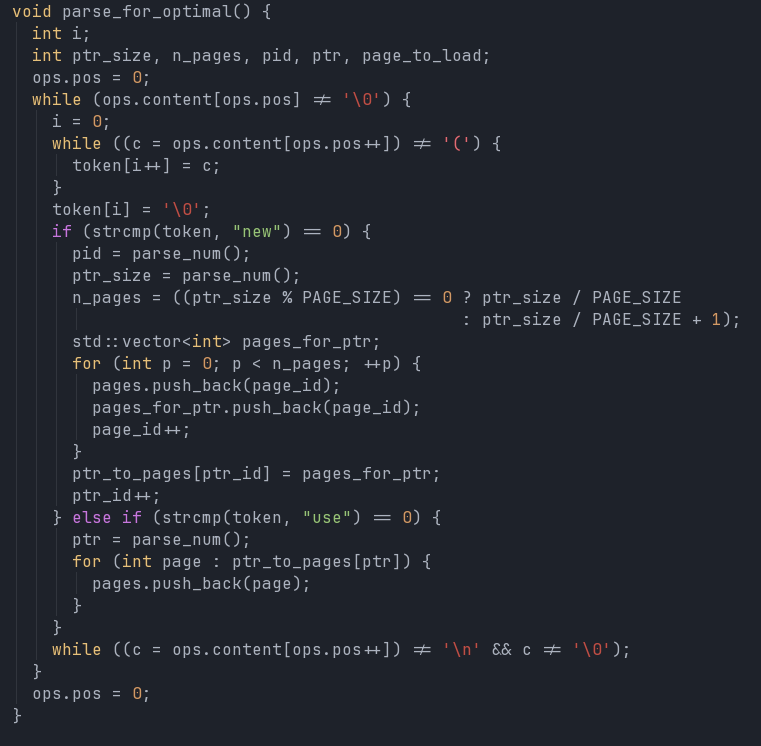
\includegraphics[width=0.8\linewidth]{figuras/parse_optimal.png}
	\caption{Imagen del parser para el algoritmo óptimo}
	\label{fig:parse_optimal}
\end{figure}

\begin{figure}[h]
	\centering
	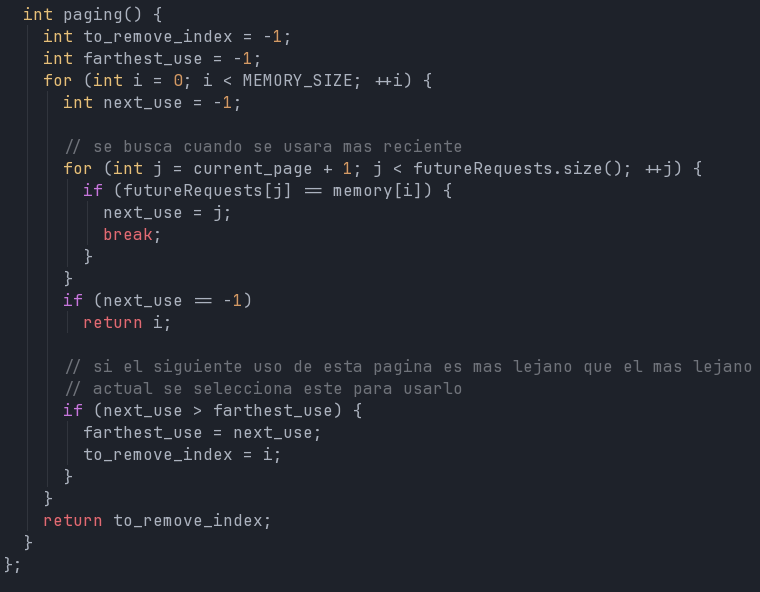
\includegraphics[width=0.8\linewidth]{figuras/optimal.png}
	\caption{Imagen del algoritmo óptimo}
	\label{fig:optimal}
\end{figure}


\subsection{FIFO y Second Chance}
\subsubsection{FIFO}
El algoritmo FIFO es (junto a Random) el algoritmo más simple impementado para manejar paginación en el programa.
Este algoritmo por sus siglas significa ``First in First Out'', como su nombre lo indica, este consiste en sacar la página que lleva más tiempo en memoria para dar espacio a las demás \cite{ref0}. \\

Para implementar esto, se decidió utilizar dos variables ``to\_remove\_index'' (el índice de la página que se va a remover) y ``time\_loaded'' (el tiempo que la página lleva cargada). 
Por defecto ambas se setean en -1, este valor es reescrito en el momento que se ejecuta la lógica del algoritmo.
Dentro de un for loop se revisan todas las páginas dentro de memoria, si la cantidad de tiempo que esa página es mayor a la cantidad guardada en ``time\_loaded'' se actualiza el índice y dicha variable.
De esta forma, una vez termina el for loop, se tiene el índice de la página que lleva más tiempo cargada, una vez hecho esto simplemente se retorna este índice.
Este comportamiento se puede ver en el código mostrado en la Figura \ref{fig:fifo}.

\begin{figure}[h]
  \centering
  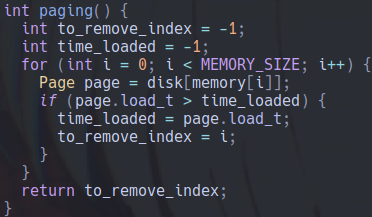
\includegraphics[width=0.8\linewidth]{figuras/fifo.png}
  \caption{Ilustración de el algoritmo FIFO}
  \label{fig:fifo}
\end{figure}

\subsubsection{Second Chance}
El algoritmo Second Chance es una pequeña mejora del algoritmo FIFO, este busca tomar en cuenta información de los usos pasados \cite{ref1}. 
Este algoritmo utiliza un bit para marcar las páginas cada vez que ocurre un HIT en esta. 
A la hora de reemplazar una página, esta trata de seleccionar la que lleva más tiempo dentro de memoria, pero si está marcada con el bit encendido, descarta esta página, expira el bit agregando un 0, y luego elige la siguiente que lleva más tiempo, repitiendo el proceso si este también tiene el bit encendido. \\

Para implementar este algoritmo se copia la memoria en un vector, luego se busca la página más reciente dentro del vector. 
Si la página más reciente no tiene el bit encendido, simplemente se retorna su índice en memoria. 
Si dicha página está marcada, se expira la marca y se saca la página del vector para no seleccionarla.
Luego se repite el proceso para seleccionar otra página. 
Si se que todas las páginas estaban marcadas, se busca la más reciente dentro de memoria.
El código que implementa esta lógica se puede ver en la Figura \ref{fig:second_chance}.


\begin{figure}[h]
  \centering
  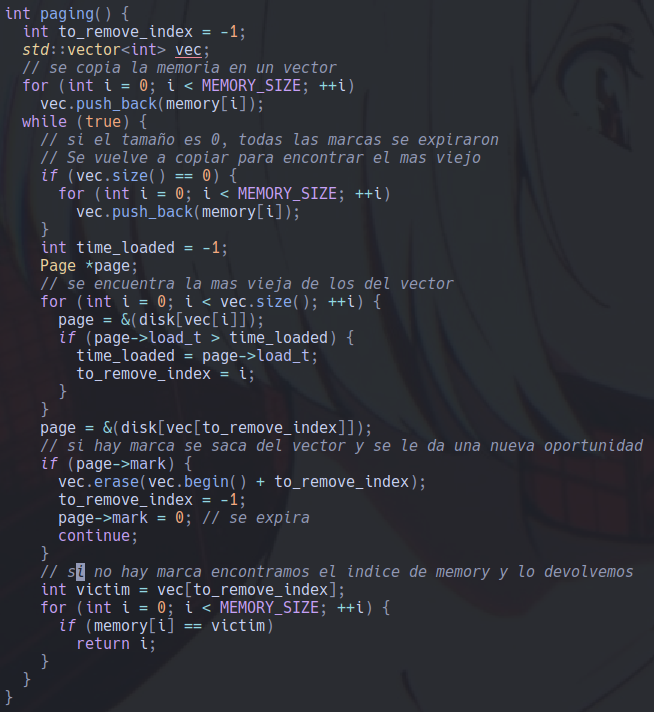
\includegraphics[width=0.8\linewidth]{figuras/second_chance.png}
  \caption{Ilustración de el algoritmo Second Chance}
  \label{fig:second_chance}
\end{figure}

\subsection{LRU y MRU}
Los algoritmos de paginación MRU(Most Recently Used) y LRU(Least Recently Used) funcionan de forma similar.  Ambos utilizan una marca de tiempo que se inserta en las páginas cuando se cargan en RAM y cuando se utilizan.  La página que se escoge para ser reemplazada es la que fue utilizada más recientemente o menos reciente, dependiendo de que algoritmo se utilice \cite{ref0}.

La implementación del MRU es simple, se trata de un algoritmo que recorre todo el arreglo de memoria para obtener que tan recientemente se usó cada página, y a través de una comparación encuentra la más utilizada recientemente (ver figura \ref{fig:mru}). La implementación del LRU es exactamente igual pero la comparación cambia para encontrar la página menos utilizada recientemente (ver figura \ref{fig:lru}).

\begin{figure}[h]
	\centering
	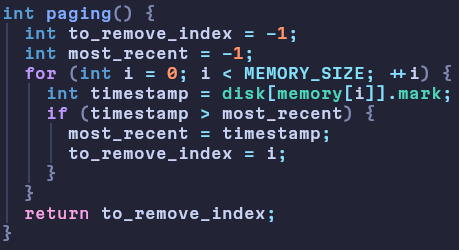
\includegraphics[width=0.8\linewidth]{figuras/mru.png}
	\caption{Imagen del algoritmo MRU}
	\label{fig:mru}
\end{figure}

\begin{figure}[h]
	\centering
	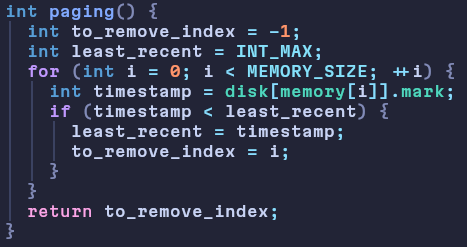
\includegraphics[width=0.8\linewidth]{figuras/lru.png}
	\caption{Imagen del algoritmo LRU }
	\label{fig:lru}
\end{figure}
  

\subsection{Random}

El algoritmo de paginación Random o Aleatorio reemplaza una página en memoria escogida de forma aleatoria, debido a esto su implementación es trivial y se limite a conocer sobre como se consiguen números aleatorios en el lenguaje escogido para implementarlo (ver figura \ref{fig:random}). En está implementación se hace usó de una semilla para poder replicar el comportamiento del algoritmo, está semilla se configura justo antes de crear el objeto Random\_MMU.

\begin{figure}[h]
	\centering
	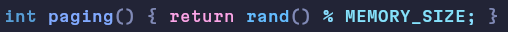
\includegraphics[width=0.8\linewidth]{figuras/random.png}
	\caption{Imagen del algoritmo Random }
	\label{fig:random}
\end{figure}



\chapter{Instrucciones}
\section{Cómo instalar el programa}
\begin{enumerate}
  \item Descargue el código fuente del programa. Puede hacerlo de las dos siguientes formas:
    \begin{itemize}
      \item Dirigirse al repositorio de GitHugitb mediante su navegador a través del siguiente link: \url{https://github.com/Andres2950/PSO\_PagingSimulator.git}
      \item Instalarlo directamente con el comando \\
    \texttt{wget \url{https://github.com/Andres2950/PSO\_PagingSimulator/archive/refs/heads/main.zip}}
    \end{itemize}
  \item Descomprima el archivo .zip descargado utilizando el comando \texttt{unzip}.
  \item Al extraer el archivo podrá observar la estructura de organización similar a la figura \ref{fig:estructura}.
\item Ejecute el archivo \texttt{install.sh}, asegúrese de qué tenga permisos de ejecución, puede utilizar el comando \texttt{chmod +x install.sh} en caso de que no los posea y luego ejecute de la siguiente forma \texttt{./install.sh}. \\
  Este archivo se hará cargo de la instalación del compilador \textit{g++} necesario para compilar el código fuente. Además hará la instalación del paquete \textit{cmake} para la ejecución del archivo ``CMakeLists.txt", dicho archivo posee las instrucciones de compilación de \textit{SDL} para resolver todas las dependencias. 
\item Note que la instalación de dichos paquetes requiere permisos de usuarios root, al ejecutar el archivo \texttt{install.sh} este se volverá a ejecutar con dichos permisos, para esto solicitará la contraseña del usuario root para tener dichos permisos de ejecución (la contraseña es totalmente invisible para el programa) y así poder descargar los paquetes.
\item La compilación de los archivos se realiza sin permisos root.
%\item Además, el \texttt{install.sh} hará una copia de los binarios \texttt{huff} y \%texttt{dehuff} en el directorio \textit{/usr/bin} de la máquina para poner ser %accedidos desde cualquier lugar y utilizado en múltiples directorios sin necesidad %de mover los archivos a comprimir o descomprimir a una carpeta en particular.

\end{enumerate}

\begin{figure}[h]
	\centering
	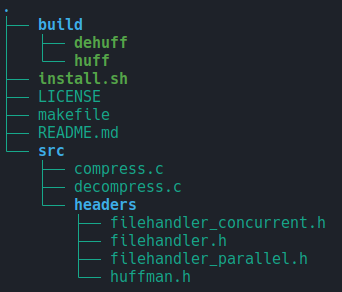
\includegraphics[width=0.8\linewidth]{figuras/estructura.png}
	\caption{Imagen de la estructura del programa }
	\label{fig:estructura}
\end{figure}

\section{Cómo utilizar el programa}
Una vez terminado el procedimiento de instalar el programa puede utilizar el comando \texttt{./build/app/app} en la carpeta del proyecto descargada para ejecutar el programa de simulación.

\chapter{Conclusiones}


% Estilo de bibliografía APA
% Si quiere usar el estilo IEEE comente esta línea
\bibliographystyle{apacite}

% Descomente esta línea para usar el estilo de bibliografía IEEE
%\bibliographystyle{ieeetr}
\bibliography{referencias}

\end{document}
